\pagebreak
\chapter{Concept \& Design Strategy}
\label{ch:concept}

\markboth{Embodied-Driven Design}{}

\begin{flushright}
\textit{
``one sees the environment not just with the eyes, but with the eyes in the head on the shoulders of a body that gets about. We look at details with the eyes, but we also look around with the mobile head, and we go-and-look with the mobile body''}
\par\hfill\textsc{James J. Gibson, The Ecological Approach to Visual Perception 1979}


\end{flushright}
\vspace{15pt}

%\section{Overview}
\begin{comment}
\begin{wrapfigure}[23]{r}{0.41\textwidth}
  \captionsetup{justification=centering}
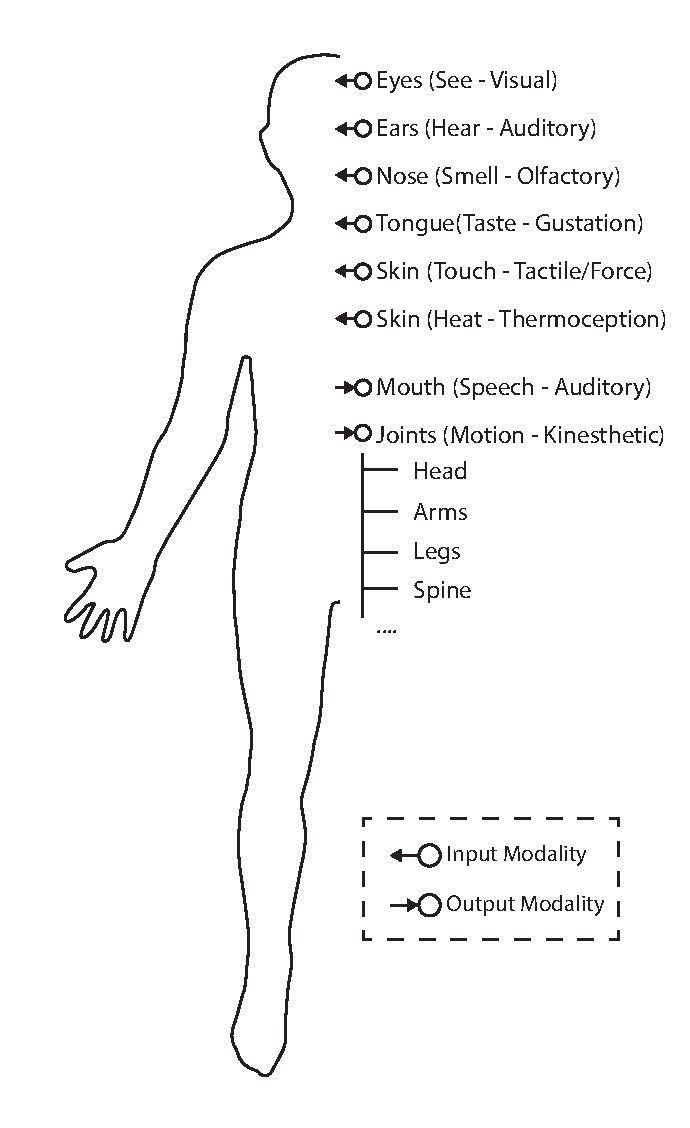
\includegraphics[width=0.35\textwidth]{figures/concept/Modalities.pdf}
\caption{Human Body Input/Output Modalities}
  \label{fig:intro-modalities}
\end{wrapfigure}


The idea of Embodied-Driven Design relies on the possibility of reconfiguring our body schema mapping and structure using mediated representation in the remote location. But before diving into the topic of body schema design and reconfiguration, a base design pattern is necessary to be described. Loosely-Couple Modalities (LCM) design pattern is the fundamental block in the design process of body schema reconfiguration. Using this design pattern, it's possible to simplify the body structure and the involved modalities in the target teleoperated task or goal representation. Using this design pattern, its possible to reconfigure the body schema using an Embodied-Driven Design framework. 

\end{comment}
%Chapter 2 has introduced the fundamental background of Embodied-Driven Design
This chapter will address the design aspects and process for body driven applications by first providing a systematic model of human body schema, and then deriving topological models for the postural and sensory body schema. The idea of decoupling and re-coupling is also discussed here as a part of LCM design pattern which allows the reconfiguration of body schema mapping by using a topology of the various body modalities. And finally, EDD framework is described along with the meta-modeling tools and modular blocks that reflects LCM design pattern. Three meta-modeling design categories are discussed that summarizes the major use-cases and design scenarios that EDD can serve. To facilitate the design process, an embodiment toolkit is proposed which can be used along with EDD framework to prototype and reflects the meta-models into a physical form.

\newpage
\section{Engineering Body Schema}
\label{sec:concept-engineering}

In order to create a system which supports the ability to modulate our sense of embodiment into a new representation, the topic of body schema is important to fundamentally analyzed and to design a systematic model that reflects the properties of the body schema. 

As described in Chapter 1, body schema is an internal/mental representation of the medium which embodies the sensory and decisions of one's self. The medium of representation holds both the kinesthetic or postural model that reflects the position of body's joints and structure \cite{holmes2004body}, and the sensory or surface model that captures the information from the surrounding \cite{macaluso2010representation}. The body schema can be considered as a collection of processes which registers the postural model and validates through capturing information from the sensory model \cite{maravita2003multisensory,haggard2005disorders}. The body schema can be attributed as being plastic, that it can be altered and modified. As an example, the use of external tools effectively alter the mental structure of the postural model and thus reflecting a modified version of the body schema from the one originally maintained, incorporating the spatial and dynamic properties of the tools \cite{berti2000far,maravita2004tools,carlson2010rapid}. 

The body schema can be characterized by the following features \cite{morasso2015revisiting}:
\begin{itemize}
\item Spatially Encoded: the body schema maintains a three-dimensional postural memory of representation's parts.

\item Distributed and Modular: it uses a process of interaction between several modules (perceptual and kinesthetic parts).

\item Inter-modality and Super-modality: the internal schema is based on the sensory integral of proprioceptive and exteroceptive information to maintain the mental representation of the body. This representation can be modulated by the sensory channels, such as vision, based on the task and the environment which the body is located at. This sensory integration has the responsibility to define a modal representation which maintaining the coherence of task operation \cite{haggard2005disorders}.

\item Plasticity: body schema maintains a short-term alteration, which is measured by the length of operation \cite{maravita2004tools}. 

\end{itemize}

%\begin{wrapfigure}[15]{r}{0.41\textwidth}
\begin{figure}[t!]
  \captionsetup{justification=centering}
  \centering
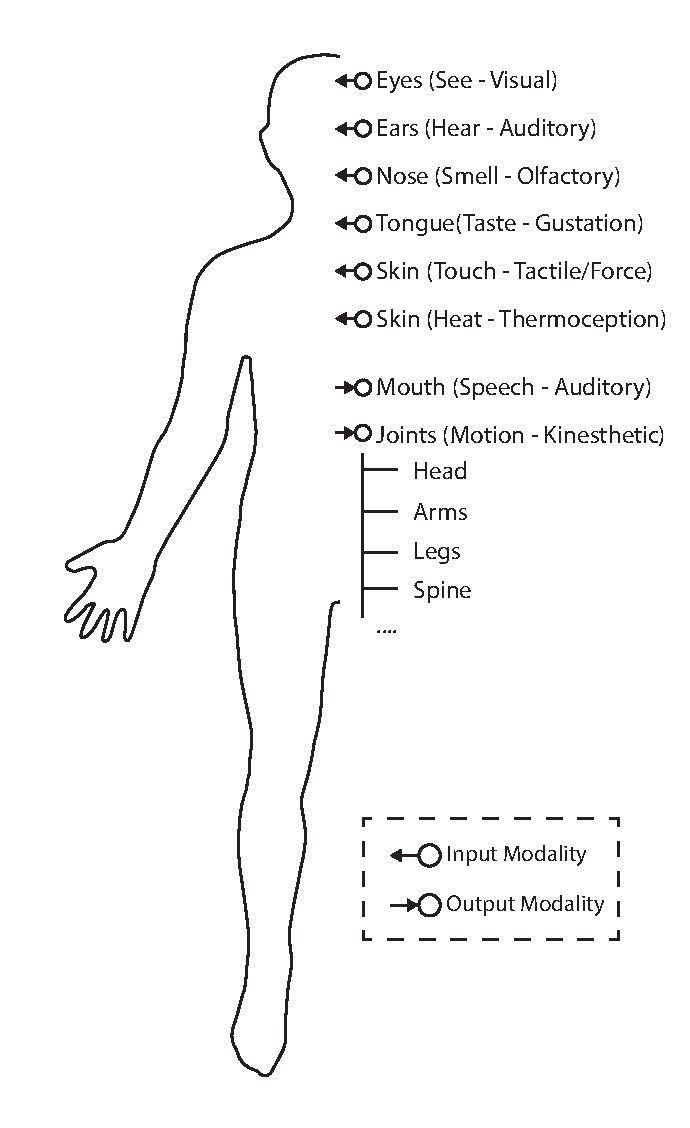
\includegraphics[width=0.6\textwidth]{figures/concept/Modalities.pdf}
\caption{Human Body Schema Input/Output Modalities Map}
  \label{fig:concept-modalities}
\end{figure}

These characteristics help to derive a systematic model of human body schema, in which the structure consists of modularized subcomponents or, as defined herein this thesis, as \textbf{Modalities}. A modality is a single component of body schema that contains an information channel as input or output which interacts with the body representation and surrounding space. \Figure{fig:concept-modalities} highlights the various modalities human body schema can be characterized with. Input modalities refer to the sensory model of human body, and output schema is related to postural model (with an exception to the speech modality).

In order to engineer body schema, and create a transfer model which alter the sense of body representation and how we interact with it, we can decouple the body schema representation into a set of modalities. In this thesis, the process of decoupling is called as ``Loosely-Coupled Modalities''.

\section{Loosely-Coupled Modalities}
\label{sec:concept-LCM}

As in our daily interaction, we rely on cross-modalities to have a clear comprehension of the tasks involved in. Human body physical structure imposes tight coupling of these modalities, and our mental representation is mapped to this tight coupling. Ability to isolate and separate these modalities can help to redesign new sort of perceptual augmentation interactions by modulating the information channels from the representation and feed them back to the human body through perceptual proxy devices (such as HMD, haptic interfaces, ... etc). 

\begin{table}[htp]
\centering
%\hspace*{-1cm}
\centerline{
\begin{tabular}{|l|l|l|l|}
\hline
\footnotesize
\rowcolor[HTML]{EFEFEF}
 \textbf{Modality} & \textbf{Data Representation} & \textbf{Capture Device} &  \textbf{Representation} \\ \hline
\textbf{Vision} & Imagery & Cameras & HMD \\ \hline
\textbf{Hearing} & Auditory & Michrophone & Speaker \\ \hline
\textbf{Speech} & Auditory & Michrophone & Speaker \\ \hline
\textbf{Kinematic} & Spatial & Motion Tracking & Servo Motors  \\ \hline
\textbf{Touch} & Vibratory Signal & Force/Tactile Sensors & Haptic Display \\ \hline
\end{tabular}
}
%\hspace*{-1cm}
\caption{Examples of human body modalities \& corresponding representations }
\label{table:concept-modalities}
\end{table}


The idea of Loosely-Coupled Modalities (LCM) resides on treating each Input/Output modality as a separate channel of interaction. LCM simplifies the body schema structure into primitive modalities, such as joints that can be represented by position and orientation, visual input for each eye, auditory input and output for the ears and the mouth, ...etc. The modalities have a predefined information type that only accepts, for example, the joints only accept spatial information but not an audio signal. \Table{table:concept-modalities} shows various modalities with the corresponding data type which accepts. A channel accessor (symbolized by a circle and an arrow) represents the information flow of the modality. Two types of accessors are defined: input and output. An input accessor directs the information flow from the representation into the body through perceptual proxies, and the output directs the internal state of the body to the representation through tracking and sensing devices. The information flow is defined by a digital form, which is sampled through capture devices, and reproduced through perceptual proxies. \Table{table:concept-modalities} lists the modalities with the corresponding representations and information type that can be used to define them.

In this thesis, the body schema modalities are categorized into two types of modalities: 
\begin{itemize}
\item Postural modalities: focuses on the spatial, three-dimensional attributes related to the body and its representation. Mainly consisting of the joints and shape of the body. 
\item Sensory modalities: contains the various sensory attributes of the human body. 
\end{itemize}

Before describing each set of modalities categorizes, the concept of decoupling and re-coupling of modalities is explained. An abstraction model of the postural and sensory modalities are defined and referred to as Topology models of human body. 

A \textit{Topology} was originally derived in mathematics from the fields of geometry and set theory which defines spatial relationships that connects the matter being studied regardless of the dimensional differences (such as length, scale, ...etc) or descriptive properties (such as color, weight, ..etc). For human bodies, two bodies would have the same topology as long as they have the same number of limbs, eyes, ears, ...etc. If a body has experienced certain deformations (such as a lost limb), then its corresponding postural or sensory topology has also been changed.

\pagebreak
\subsection{Postural Modalities Topology}

In order to create a model defining the body structure, a hierarchical model describing the distribution of the joints in the human body is defined. \Figure{fig:intro-BodyTopology} provides an approximation of the body joints topology. In this model, the following region categories are used:

\begin{figure}[b!]
  \centering
  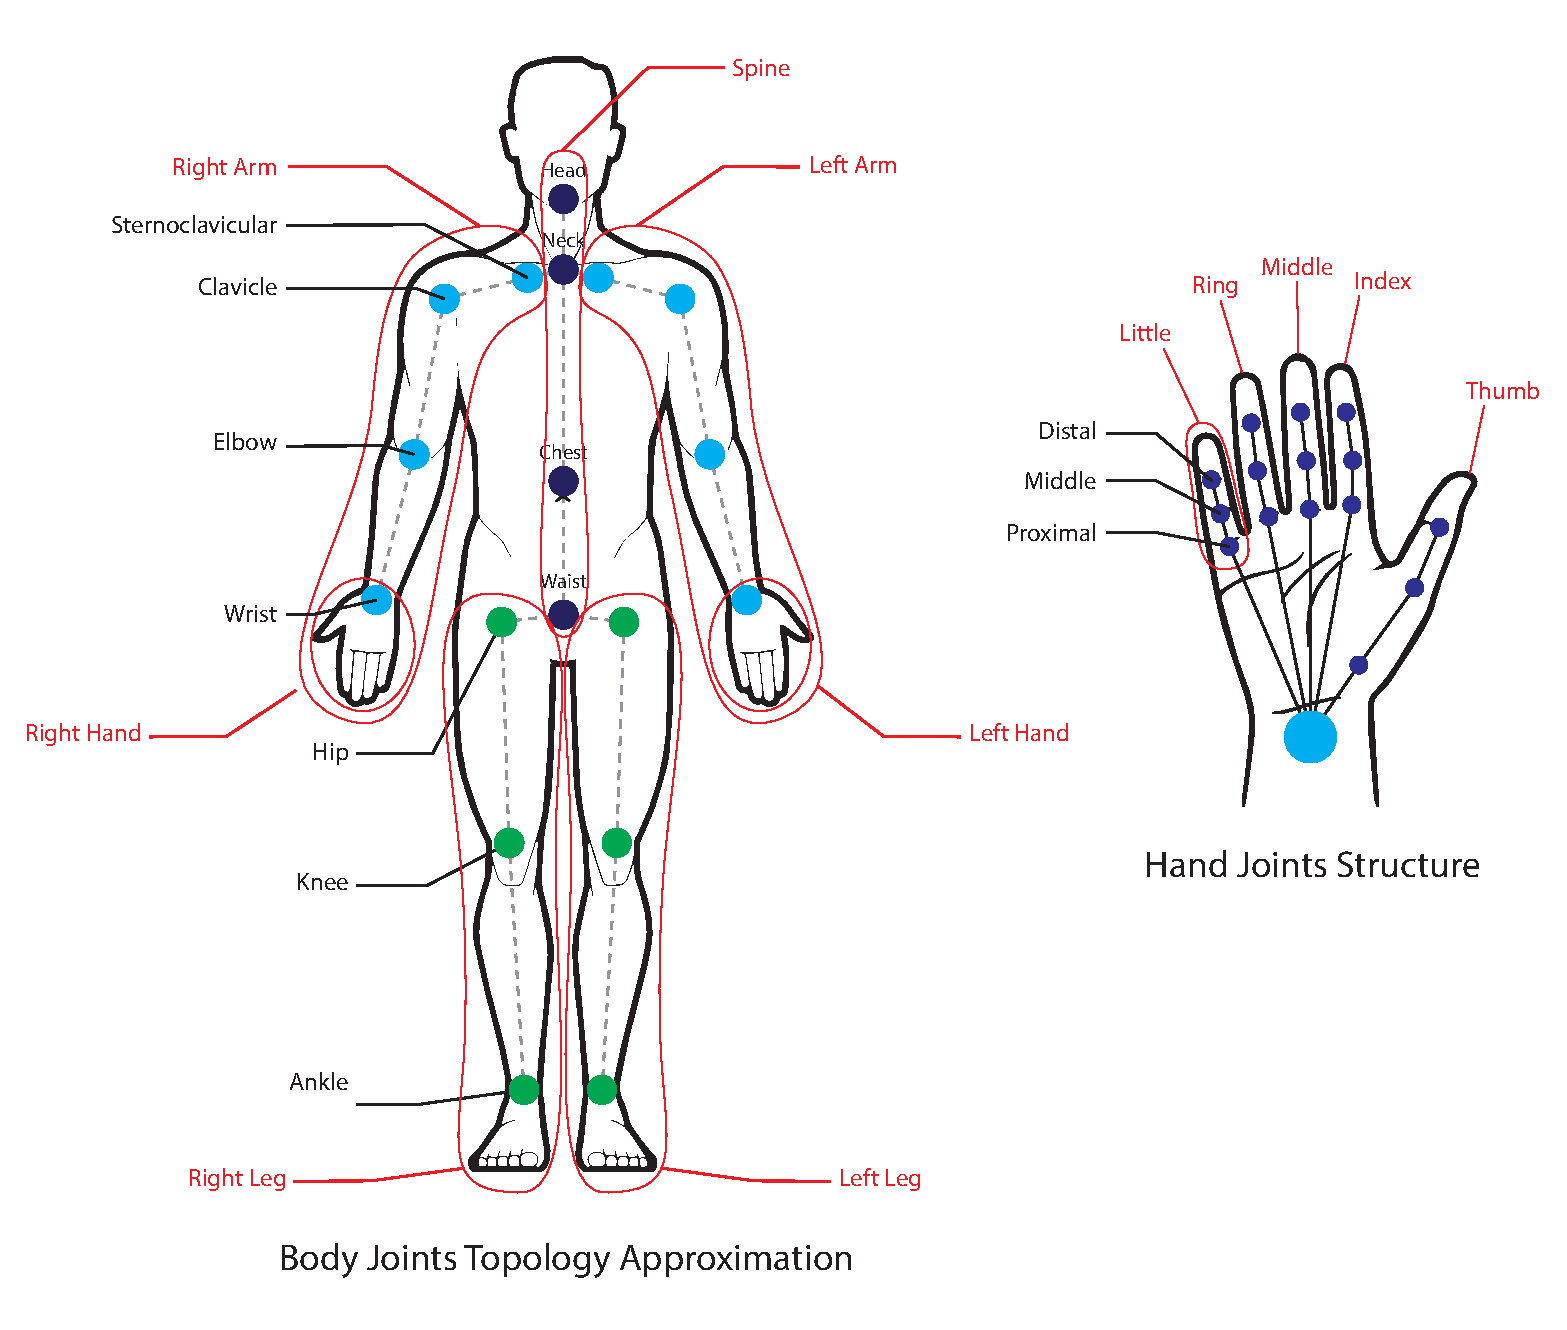
\includegraphics[width=1\linewidth]{figures/concept/BodyTopology.pdf}
  \captionsetup{justification=centering}
  \caption{Body joints topology approximation diagram, and hand joints structure.}
  \label{fig:intro-BodyTopology}
\end{figure}

\begin{itemize}
\item \textbf{Spine Region}: Contains the vertebral column joints which control the overall orientation of the body. The human spine structure consists of 33 vertebrae joints \cite{drakemitchell}, the first 9 joints (from the bottom) are fused into two regions: Coccyx (4 vertebrae), and Sacrum (5 vertebrae). The rest of joints contributes mainly in the motion. Instead of modeling the 24 joints, they were categorized into three regions: Lumbar spine (5 vertebrae) mapped into the Waist, Thoracic spine (12 vertebrae) mapped into the Chest, and Cervical spine (7 vertebrae) mapped into the Neck. Lastly, to provide an individual control to the head, an extra joint to the structure is added as Head.

\item \textbf{Arm Region}: Has the structure of the human arm, and it consists of four joints in total to define the motion of the arm: Sternoclavicular joint, Clavicle joint, Elbow joint, and Wrist joint. The arm also contains a sub-region defining the hand.

\item \textbf{Hand Region}: A sub-region which belongs to the Arm region. Contains the definition of hand joints structure. The hand region is defined by 5 fingers, each finger has the following structure:
\begin{itemize}
  \setlength\itemsep{0em}
\item Proximal Joint: the base joint of the finger.
\item Middle Joint: the second joint of the finger.
\item Distal Joint: tip joint of the finger.
\end{itemize}

\item \textbf{Leg Region}: Defines a general structure of the human leg, and consists of three joints: Hip joint, Knee joint, and Ankle joint.
\end{itemize}


Using the previous categories, it's possible to define a postural body schema as: Spine, Left Arm, Right Arm, Left Leg, and Right Leg. In total, the number of joints defined by this approximation is: 
\begin{equation}
\begin{split}
Joints\ count &=Spine + 2\times (Arm+Hand)+2\times(Leg) \\
&=4 + 2\times(4+15)+2\times3\\
&=48\ joints
\end{split}
\end{equation}

The joint, which is considered as the minimal, atomic representation for postural modality, is defined using two attributes:
\begin{itemize}
  \setlength\itemsep{0em}
\item Position: 3 axis (X,Y,Z) tuple defining joint's spatial position.
\item Orientation: a quaternion defining the direction of the joint. 
\end{itemize}

\pagebreak
\subsection{Sensory Modalities Topology}

\begin{figure}[b!]
  \centering
  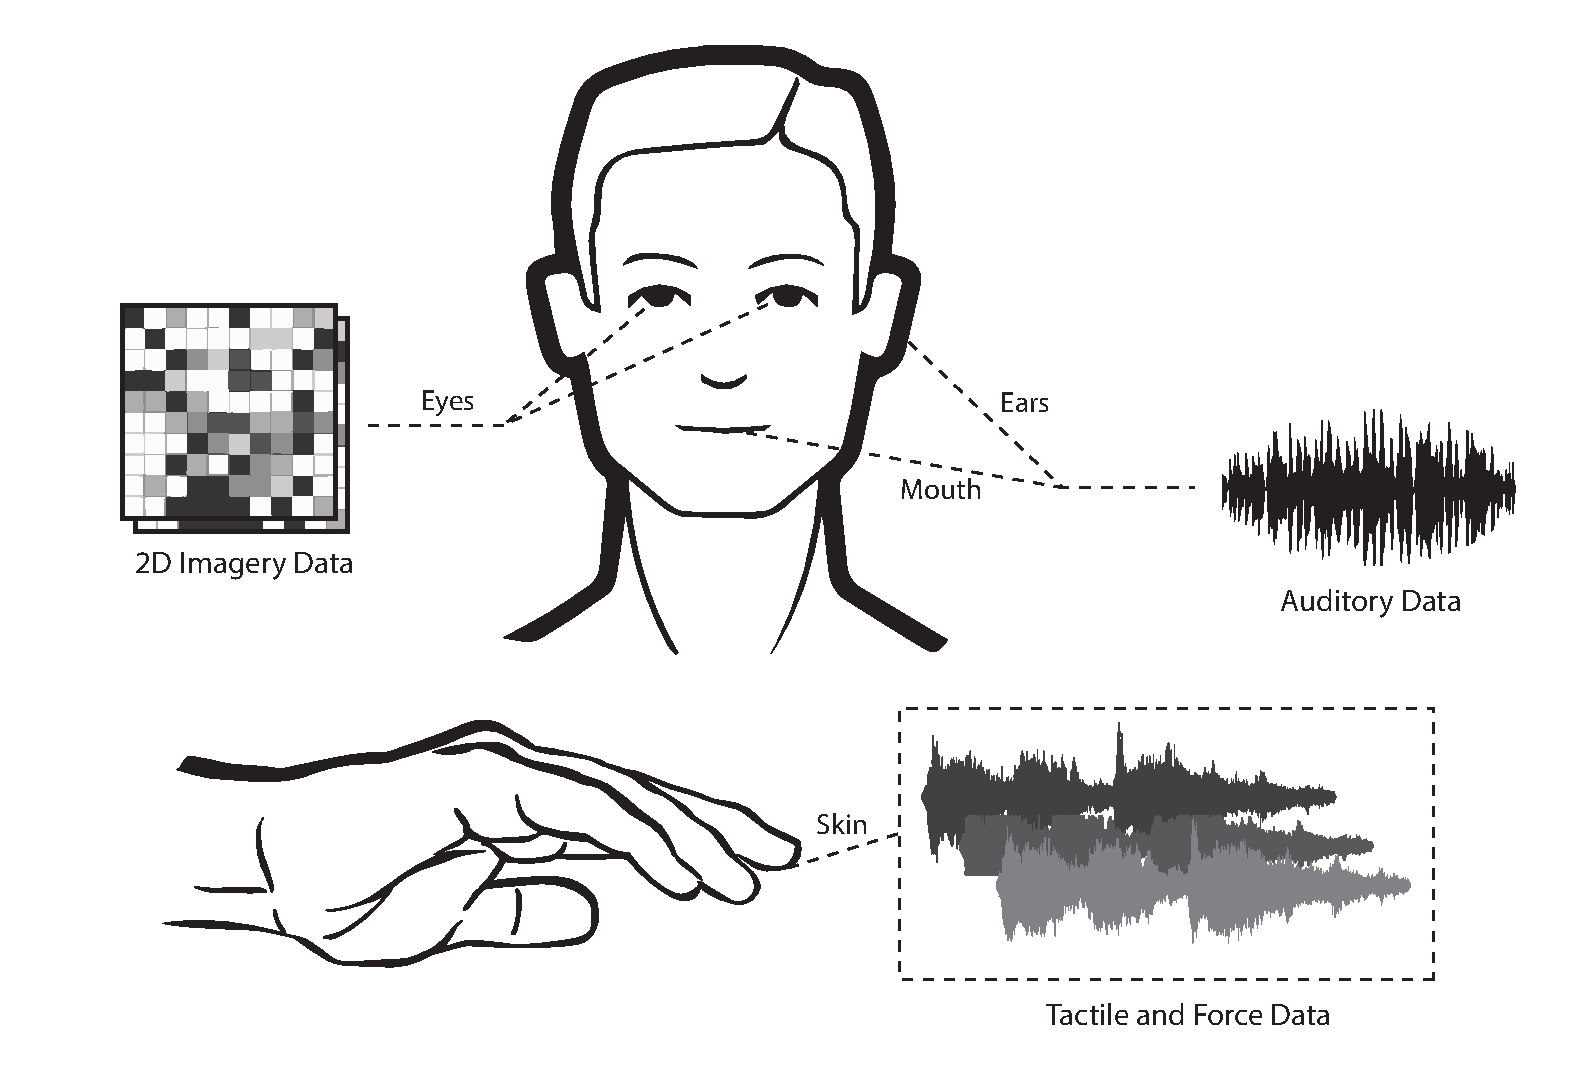
\includegraphics[width=1\linewidth]{figures/concept/PerceptualDataType.pdf}
  \captionsetup{justification=centering}
  \caption{Sensory modalities categorization with their data type.}
  \label{fig:concept-SensoryModalities}
\end{figure}

For the perceptual schema of the body, major sensory modalities are characterized based on their function and data type. \Figure{fig:concept-SensoryModalities} highlights four different types of perceptual modalities with their corresponding data they accept. The sensory modalities considered in this thesis are as follow:

\begin{itemize}
  \setlength\itemsep{0em}
\item \textbf{Eyes}: provide the visual feedback to the user. Consists of two channels: left and right eye. Data type they accept is 2D image data.

\item \textbf{Ears}: provide auditory feedback, and consists of two channels: left and right ear. Corresponding data type is audio signal (sampling rate 44100Hz or higher).

\item \textbf{Mouth}: captures the speech audio of the user. A single data channel with data type of audio signal (sampling rate 44100Hz or higher).

\item \textbf{Skin}: provides tactile and force feedback. Number of channels is defined based on the model (spatial resolution). Accepted data type is a vibrotactile signal.
\end{itemize}

These modules provide the sensory mapping for the human body. The use of digital data as input/output helps to transmit and alter the sensory information using computer mediated communication between the human operator and his representation(s).

\subsection{Decoupling and Re-coupling of Modalities}

In order to simplify the process of modeling the interactions of body schema, the various modalities described previously should use a hierarchical structure to access a region of modalities or the individual atomic level of each sub-modality. 

\begin{wrapfigure}[20]{l}{0.4\textwidth}
  \captionsetup{justification=centering}
  \centering
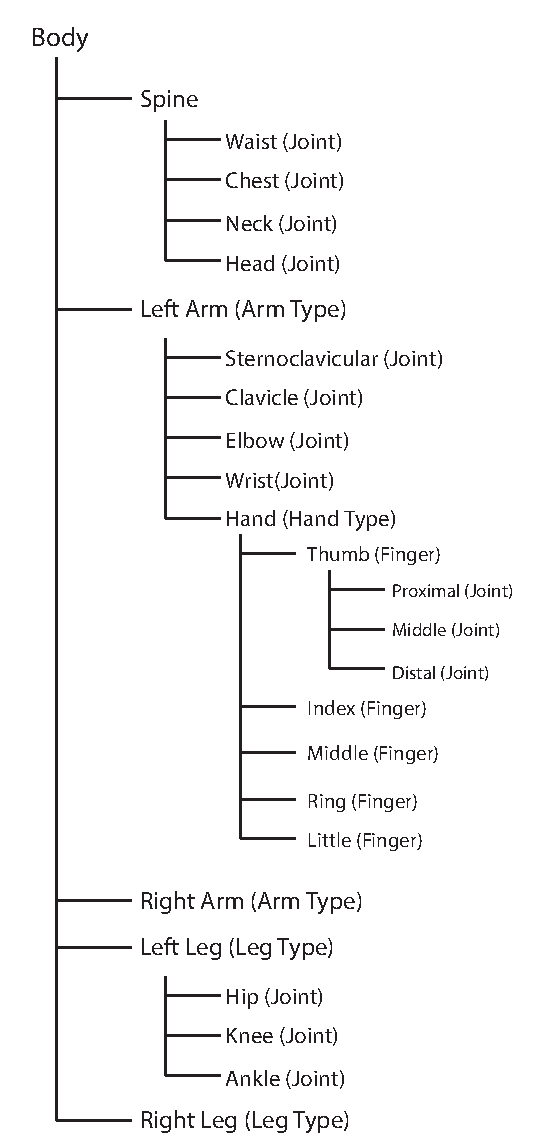
\includegraphics[width=0.4\textwidth]{figures/concept/PosturalSchema.pdf}
\caption{Postural schema hierarchy}
  \label{fig:concept-postural}
\end{wrapfigure}

The use of decoupling/re-coupling in postural schema modeling, it is possible to work at any level of the body structure to map or control the motion of the regions or individual joints \Figure{fig:concept-postural}. For example, its possible to map one arm to another directly, which results to mapping the individual joints of one arm to the corresponding joints of the other joint. Or it is possible to decouple the region into its atomic structure (joints), and reassign them to a different joint, for example controlling the thigh joint using wrist joint. Similarly, for the sensory schema modeling, the stereo eyes can be decoupled into individual left and right eye which are considered the atomic level of visual modalities, and mapped to different sources. The ears can be decoupled to left and right ear, and processed individually.

%\pagebreak
\section{Body Schema Desgin}
\label{sec:concept-bodyschema}

\subsection{Model Oriented}
%express the idea of embodiment using soft representation, and ability to experience it using a physical/virtual representation
%combination of representation and virtual/visual design tools

Embodied Driven Design (EDD) aims to provide a systematic, designer-oriented, human driven body schema design and mapping. By using the idea of loosely-coupled modalities described in the previous section, body schema can be remodeled based on an alternative representation. EDD is based on two design models which defines the target application:
\begin{enumerate}
  	\setlength\itemsep{0em}
\item \textbf{Representation:} The representation of the modalities using physical and virtual means, such as robotic avatar, virtual body, non-humanoid representation, ...etc.
\item \textbf{Meta-Model:} An abstraction of the relationships between the modalities of human body and their corresponding representations. The meta-model defines a transfer function of the schema that can be direct channel mapping, or alternates the information flow of the modalities with their representations.
\end{enumerate}


\begin{figure}[b!]
  \centering
  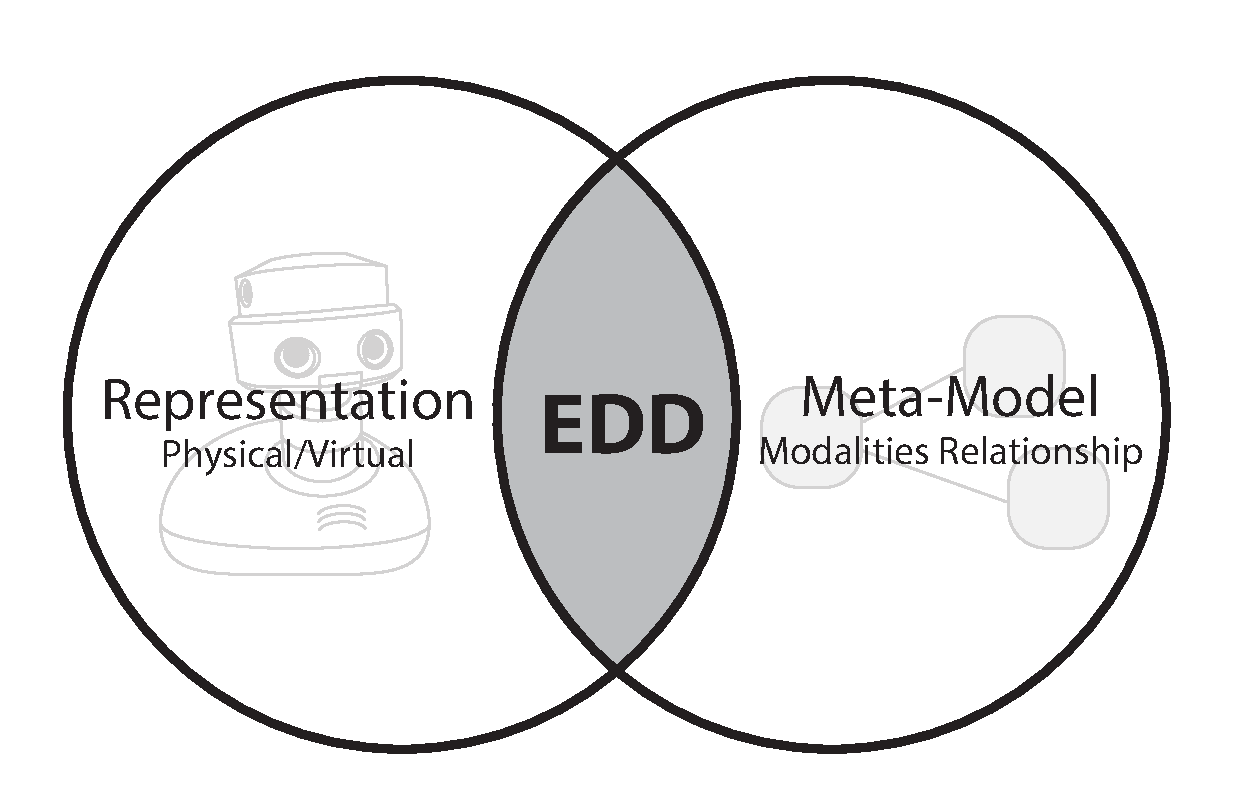
\includegraphics[width=0.8\linewidth]{figures/concept/EDD.pdf}
  \captionsetup{justification=centering}
  \caption{Embodied-Driven Design framework areas.}
  \label{fig:concept-EDD}
\end{figure}


\begin{comment}
\begin{figure}[htpb]
  \centering
  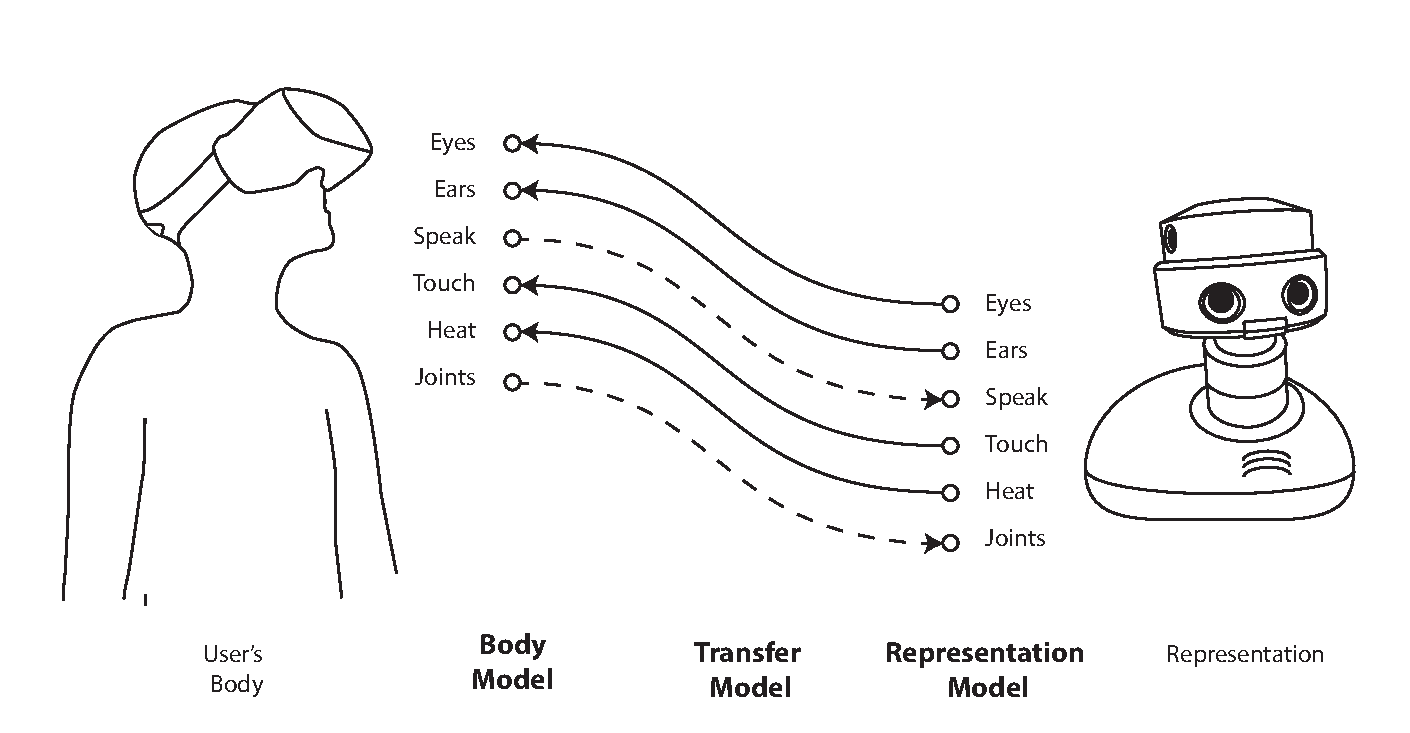
\includegraphics[width=1\linewidth]{figures/concept/EDD-Tx.pdf}
  \captionsetup{justification=centering}
  \caption{An example of EDD for direct one-to-one Telexistence mapping.}
  \label{fig:intro-EDD-TX}
\end{figure} 

\end{comment}


The overlapping of these two regions defines EDD framework \Figure{fig:concept-EDD}. Using such tools of body and representation abstraction, its possible to design new body mapping. A meta-model defines the channel flow between the various modalities that represents the user body in relationship to a representation. As shown in \Figure{fig:concept-EDD-MetaModel}, the meta-model consists of three sets of schematic models:

\begin{itemize}
  \setlength\itemsep{0em}
\item \textbf{Perceptual Model}: provides an abstraction of user's body and reflects its state into the meta-model. Contains blocks that interacts with the user's body modalities via perceptual proxies devices.
\item \textbf{Transfer Model}: an intermediate model residing between the perceptual and representation models. Contains various set of blocks that manipulates the information flow of the used modalities.
\item \textbf{Representation Model}: an abstraction of the representation used (physical or virtual). The blocks contained in this model exchange the information flow from/to the perceptual and transfer models with the used representation. Set of communication channels (e.g. network) exchange the information flow between the model and the actual representation.
\end{itemize}

\begin{figure}[t!]
  \centering
  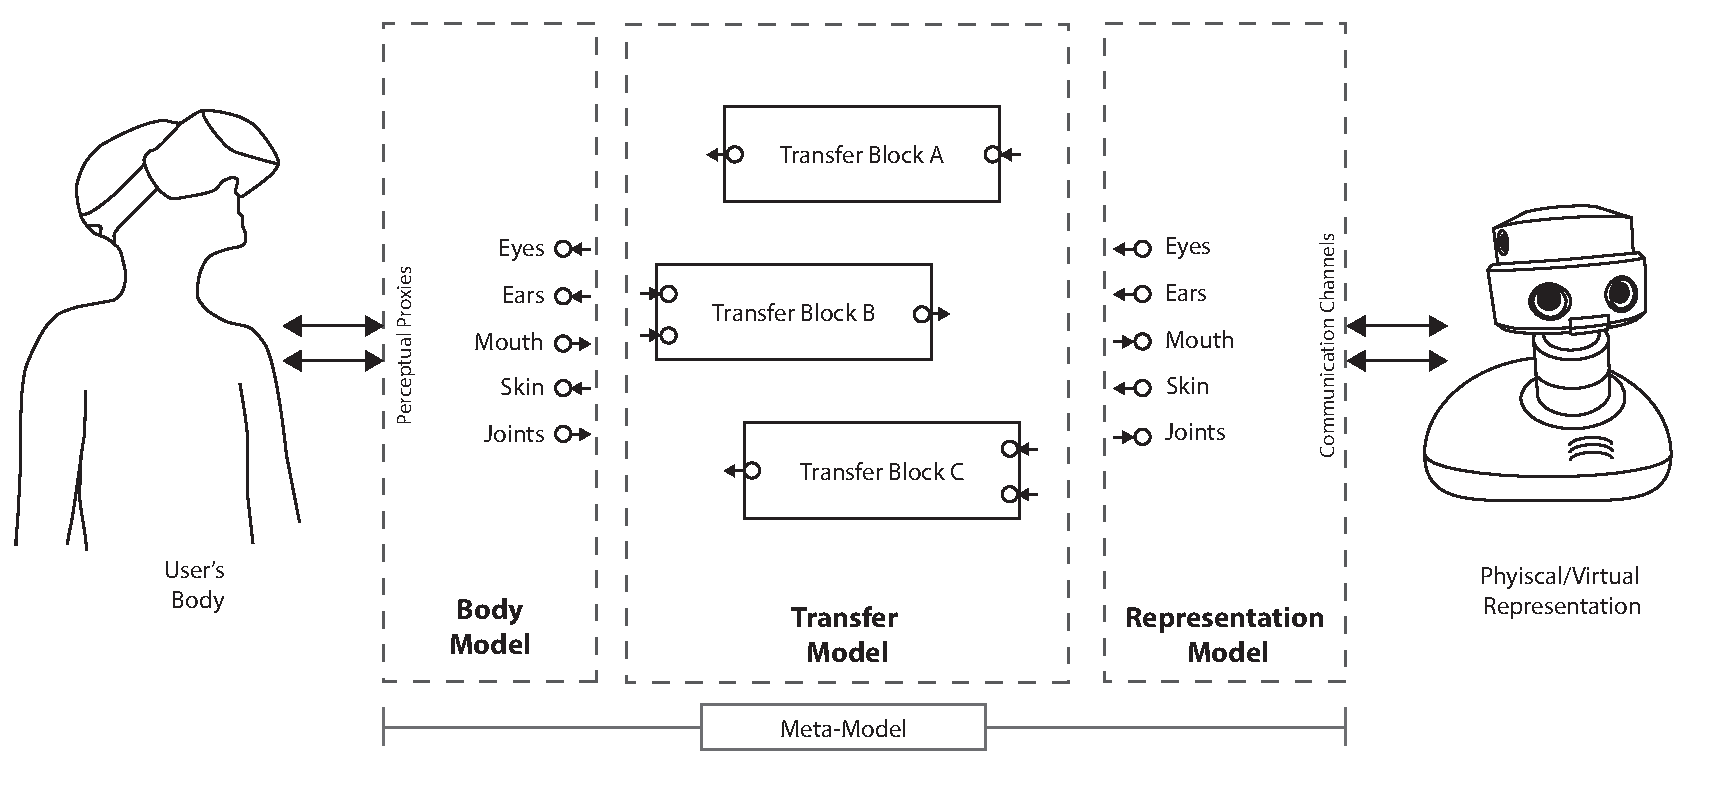
\includegraphics[width=1\linewidth]{figures/concept/EDD-metamodel.pdf}
  \captionsetup{justification=centering}
  \caption{An overview of a general EDD meta-model.}
  \label{fig:concept-EDD-MetaModel}
\end{figure}

Using these three types of models, its possible to define the flow of modalities information of the system. If the transfer model was not used, then a direct schema mapping between user's body and an avatar representation can be defined. As an example of direct schema mapping, Telexistence systems case shown in \Figure{fig:concept-EDD-TX} reflects one-to-one sensory and postural mapping configuration. Since the representation robot offers exact body schema modalities to the user, thus no intermediate transfer blocks are required and the flow between user/representation is direct. 

\begin{figure}[t!]
  \centering
  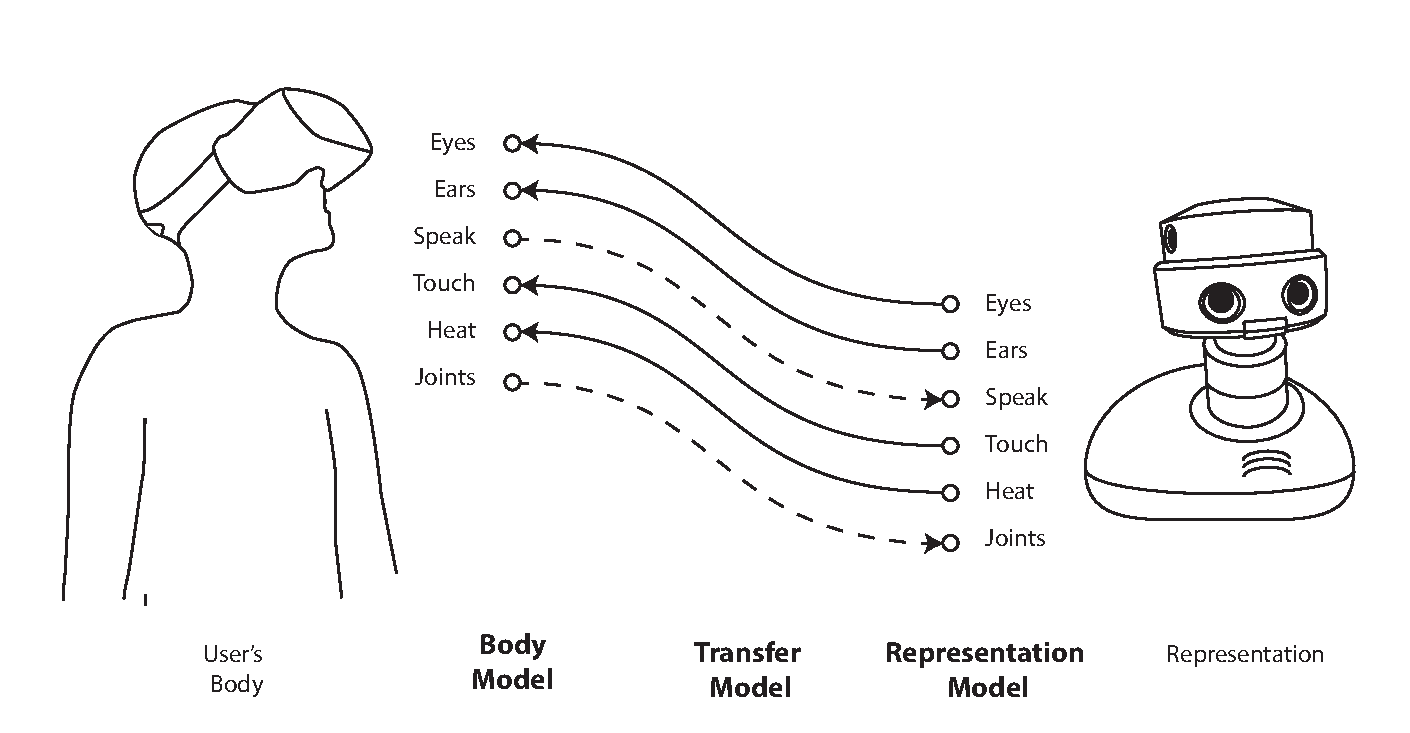
\includegraphics[width=1\linewidth]{figures/concept/EDD-Tx.pdf}
  \captionsetup{justification=centering}
  \caption{An example of EDD for direct one-to-one Telexistence mapping.}
  \label{fig:concept-EDD-TX}
\end{figure} 

%In the following section, further description about meta-modeling design process is described. Before presenting the models, two definitions related to EDD are to be explained: Blocks Categories, and Design Roles.

\subsection{Deriving LCM: Modular Blocks}%Blocks Categories

In order to reflect LCM design pattern of body schema in EDD, each or the three models defines its own set of blocks that handles separate types of modalities and information flow. The following blocks categories define the overall formats that can be used within EDD modeling:

\begin{itemize}
  	\setlength\itemsep{0em}
\item \textbf{Perceptual blocks:} driven from the user postural and sensory modalities such as vision, auditory, tactile, motion, ...etc. Inputs/Outputs of these blocks are used with the perceptual proxy devices (HMD, motion trackers, ...etc). 

\item \textbf{Transfer blocks:} acts as a function for the modalities, in which they transform or alter the data flow between the perceptual and representational blocks. Using these blocks, its possible to alter the limits of certain modalities, augment perceptual modalities, ...etc.

\item \textbf{Representation blocks:} representation dependent blocks, defines the interface and data flow between the used representation (physical, virtual, or both) and the rest of the model.

\end{itemize}


\subsection{EDD Knowledge Areas}
\label{concept:EDDKnowledgeArea}
\begin{figure}[b!]
  \centering
  \captionsetup{justification=centering}
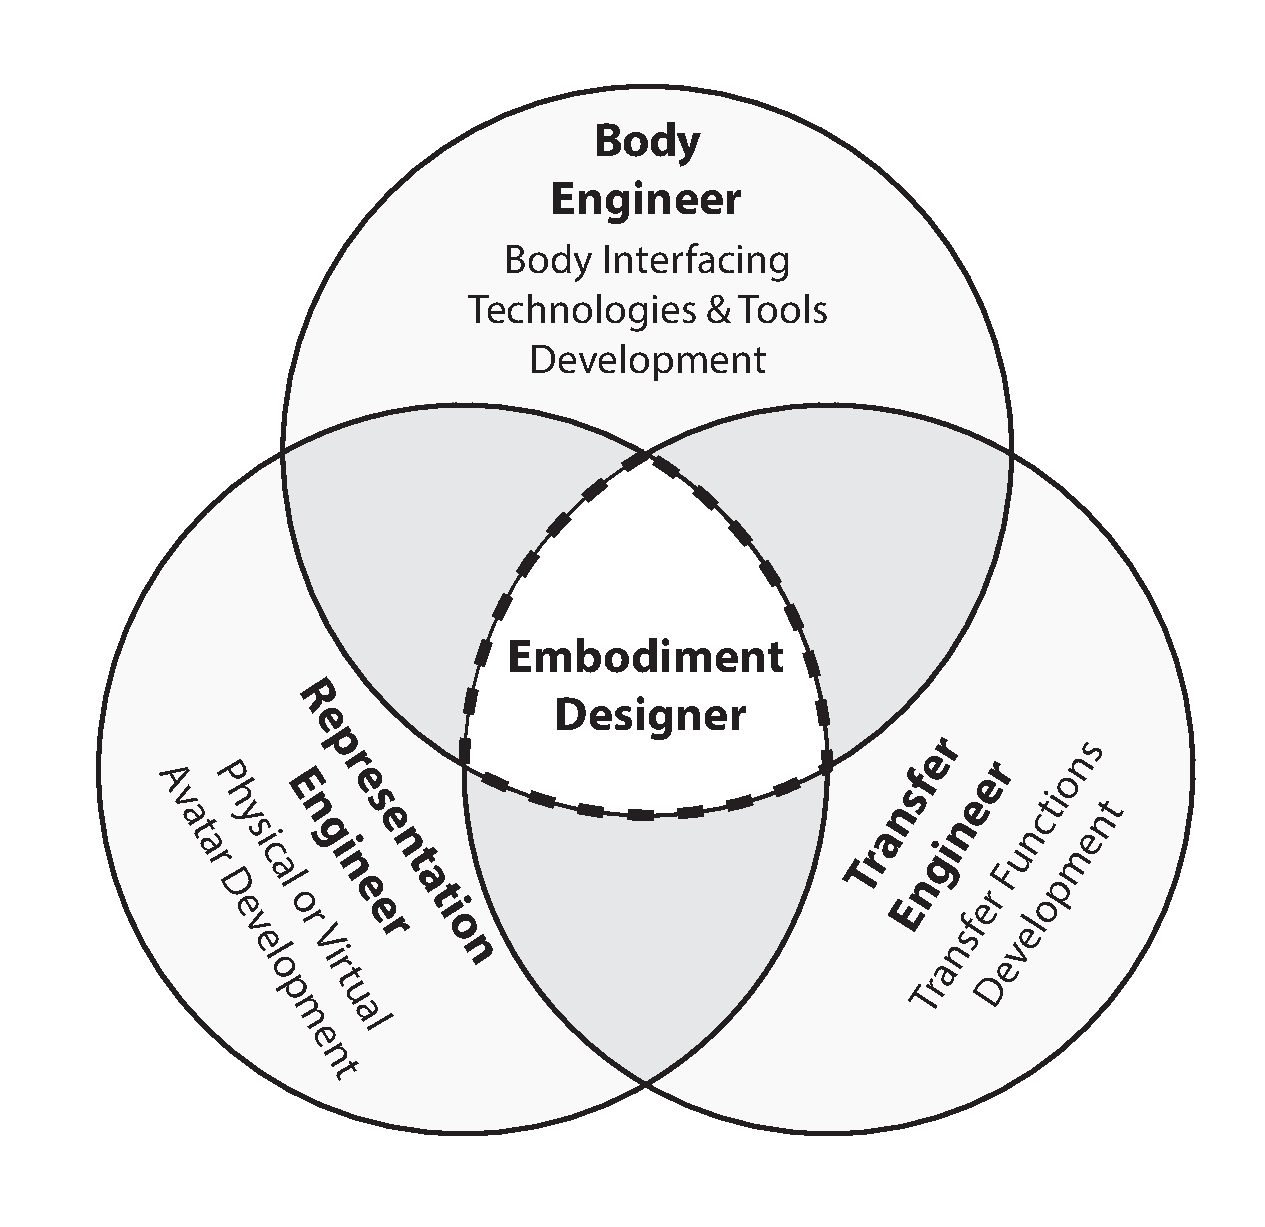
\includegraphics[width=0.6\textwidth]{figures/concept/Roles.pdf}
\caption{EDD Areas of Knowledge}
  \label{fig:concept-roles}
\end{figure}

In this proposal, four areas of knowledge (illustrated in \Figure{fig:concept-roles}) collaboratively contribute to the design process of EDD meta-models, and described as follow:

\begin{itemize}
  	\setlength\itemsep{0em}
\item \textbf{Body Engineer:} a person who uses or develops perceptual proxies and focuses on the experience provided to the user (feedback, tracking method, ..etc). This role is responsible to define and create the perceptual blocks needed in the body model side.

\item   \textbf{Representation Engineer:} this role is responsible on creating the representation blocks used for the target body schema, such as a robotic or virtual representation. 

\item  \textbf{Transfer Engineer:} a role to define and create transfer blocks used to alter the representation or the perceptual blocks. The transfer blocks defined should similar data representation for the other modalities used in the model.

\item  \textbf{Embodiment Designer:} this person creates the overall experience, that is, to use the three types of blocks to define a new body schema. The embodiment designer has an overall knowledge of the perceptual,representation, and transfer blocks to be used. The result is a meta-model designed based on the specific application.
\end{itemize}

In respect of each of the three engineering roles listed above, the meta-modeling process can be more dependent on one role than the other. In the following section, Meta-Models Categories, further description of the use-cases and scenarios in which EDD modeling process contributes into.

%(A), in Another example of EDD for body schema representation is shown in \Figure{fig:intro-EDD-TX} (B), in this case a layered perception module helps to break the one-to-one body constraint mapping to become one-to-many mapping. The module has the responsibility to provide valid perceptual input to the user. 


%\subsection{Sensory Channels Mapping}


\section{Meta-Models Categories}
\label{sec:concept-metalmodel}

Designing a presence or embodied experience requires defining the scope of the application needed, and the corresponding representation and perceptual proxies used. Representation design reflects the modalities which the used representation model affords. The representation exposes these modalities as a set of blocks that can be used in the model. The meta-model defines the connection between these modalities, and user's perceptual modalities through a mediated transfer model. 

Four categories are described here that summarizes the general usability of EDD meta-modeling for overcoming certain physical limitations, or body limitation using a representation. These meta-models describe design patterns for body mapping and configuration, and can be used individually or combined within the same meta-model.

\subsection{Direct Body Transfer}
\label{sec:concept-direct}

In this meta-modeling category, the model directly maps body modalities with the corresponding representation's modalities. \Figure{fig:concept-EDD-Direct} shows an overview of a meta-model mapping. The modalities can be directly connected to the corresponding ones, or can a transfer block could be used to alter the data (for example visual enhancement blocks, audio filter blocks, motion gain blocks, ...etc). This meta-model is generally used for cases in which there is no need to change or alter the topology of the body, and the required application requires minimum adaptation time to the representation. As an example, Telexistence systems use direct body transfer so the user can immediately use the representation (or the avatar).

This meta-model is commonly used along the other meta-models to maintain certain modality mapping without alteration.

\begin{figure}[h!]
  \centering
  \captionsetup{justification=centering}
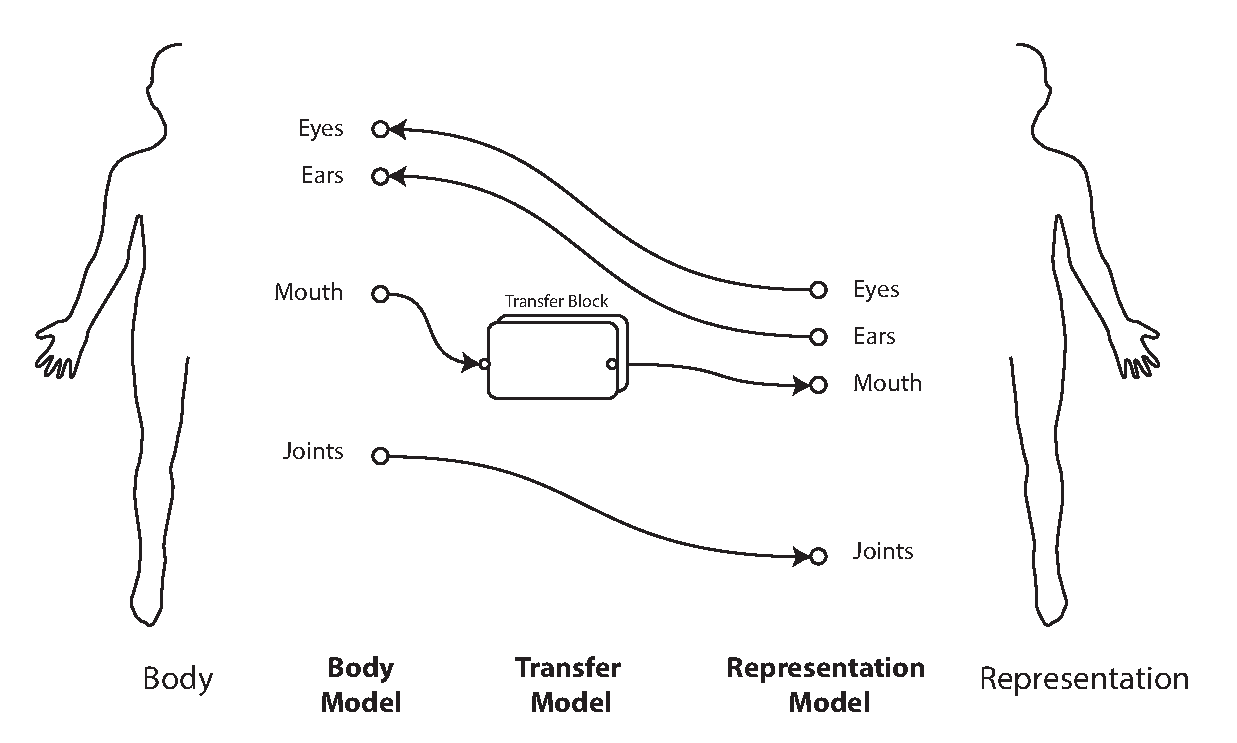
\includegraphics[width=1\textwidth]{figures/concept/EDD-Direct.pdf}
\caption{Direct body transfer meta-modeling.}
  \label{fig:concept-EDD-Direct}
\end{figure}


\subsection{Representation alteration}
\label{sec:concept-RepAlt}


Our bodies are physically limited, and our reaching space is predetermined by the length of the arms for example. Same case is reflected when operating a remote avatar with physical arms, the same physical limitations are presented. In contrast, virtual reality can easily overcome such limitations since objects in these environments are not represented using tangible materials, but instead, a digital body representation can be used.  

Representation alteration design category focuses on redefining the physical representation which can have different properties than what our bodies can provide using a hybrid virtual/physical model of human body. In this design approach, only certain modalities are physically represented (such as vision and auditory modalities) depending on the application, and other modalities are virtually defined. For example, providing a different body visuals or size than the actual. 

\begin{figure}[h!]
  \centering
  \captionsetup{justification=centering}
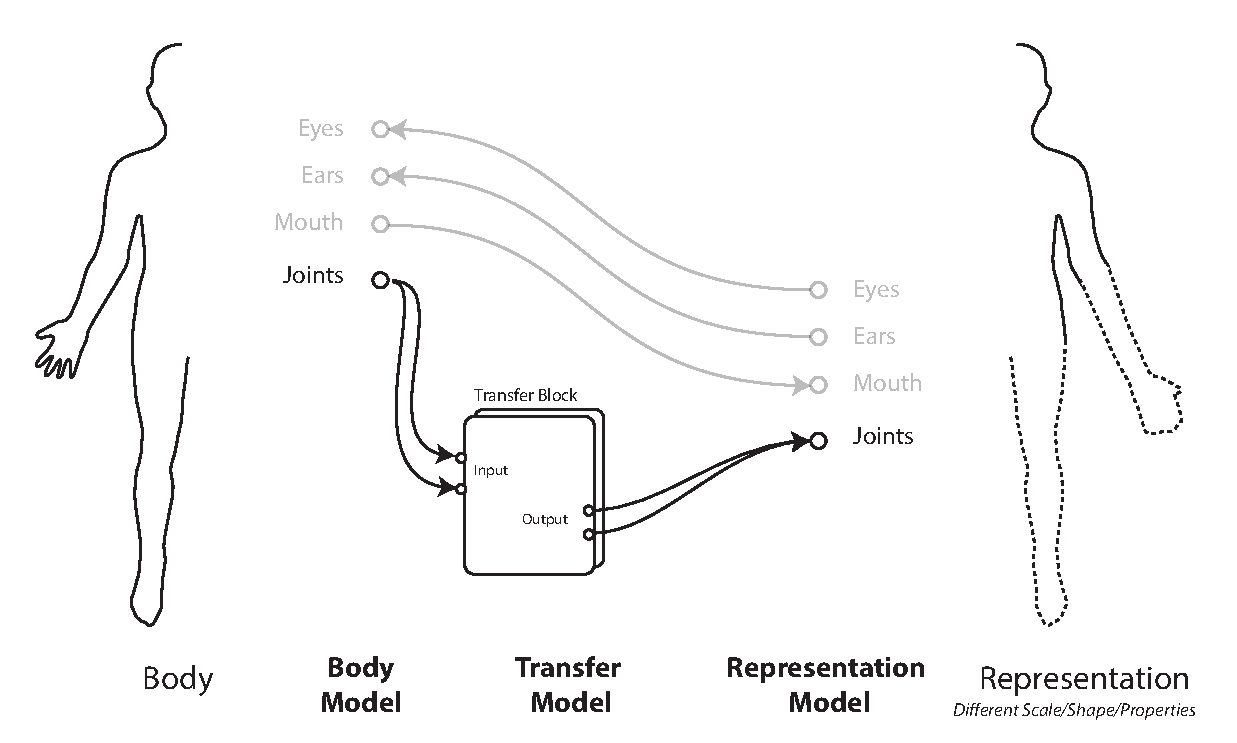
\includegraphics[width=1\textwidth]{figures/concept/EDD-RepAlt.pdf}
\caption{Representation alteration meta-modeling.}
  \label{fig:concept-EDD-RepAlt}
\end{figure}


%In order to maintain natural operation while using representation alteration design, the system should preserve operator's body visual representation both locally and remotely, also to provide mutual presence of user's interaction, the system should also presents operator's body visuals remotely. 


To visualize the representation alteration, \Figure{fig:concept-EDD-RepAlt} shows an overview of this meta-model. The representation has different attributes than the human body has, and can be represented by a hybrid physical/virtual body. For example, the representation can have different arm length than the body has, or dynamically changing its length. The mapping between the body and the representation is altered using transfer blocks that, for example, calculates the required trajectory of the representation body, and maps into the new limbs. Although the body shape changes, its topology is maintained without any alteration.

%To address the previous points, first a hand tracking device is required in order to capture user's hand visuals and motion relatively to his eyes so the eye-to-hand vector can be reconstructed at the robot side (\textit{Perceptual engineer}). Also, the body representation requires to provide visuals of the hands as being projected. To address this, a projector can be embedded into the robot which can reproduce the images of user's hands remotely (\textit{Representation engineer}). The overall system then can be modeled through EDD reflecting the components interacting between the user and the hybrid representation. \Figure{fig:concept-EDD-Mutual} shows the meta-model of this system which combines both transfer and representation blocks. As can be seen, the representation blocks does not directly map into the modalities offered by the user (virtual hands and wheels motion), and some modalities from user's side require transfer blocks to be used in the representation. The virtual hands block requires at the representation side displays user's hands remotely, and thus it requires hands image information. For this, a transfer block is used as [Hand Segmentation]. Also, in this representation, wheels are used for navigation and would require a motion vector to drive. The postural schema is different from user's schema, and thus another transfer block is also required [Motion Control].

%In the user side, the hands are captured using a first point of view (FPV) tracking camera mounted on the front of the HMD. The output of this camera is provided through the [Hands] block which is part of the postural schema of user's body. This block is linked to [Hand Segmentation] block which is responsible to extract hands information. The output of this block is mapped to [Virtual Hands] block which is used by the representation to project hands visuals. For [Motion Control] block, a body as a joystick concept can be used to drive the robot. [Motion Control] block receives head motion, and based on it calculate the motion speed and rotation which is linked to the [Wheels Motion] block to drive the robot's wheels.

In summary of Representation alteration modeling category, the design process for this meta-model is mainly derived from the body limitations. By altering the representation, and reflecting this alteration into a set of meta-modeling blocks, it's possible to match them with the modalities provided by the perceptual model.

\subsection{Topology Reconfiguration}
\label{sec:concept-OpAlt}
% \protect\footnote{Relevant work by the author \cite{saraiji2015hug}}}


\begin{figure}[b!]
  \centering
  \captionsetup{justification=centering}
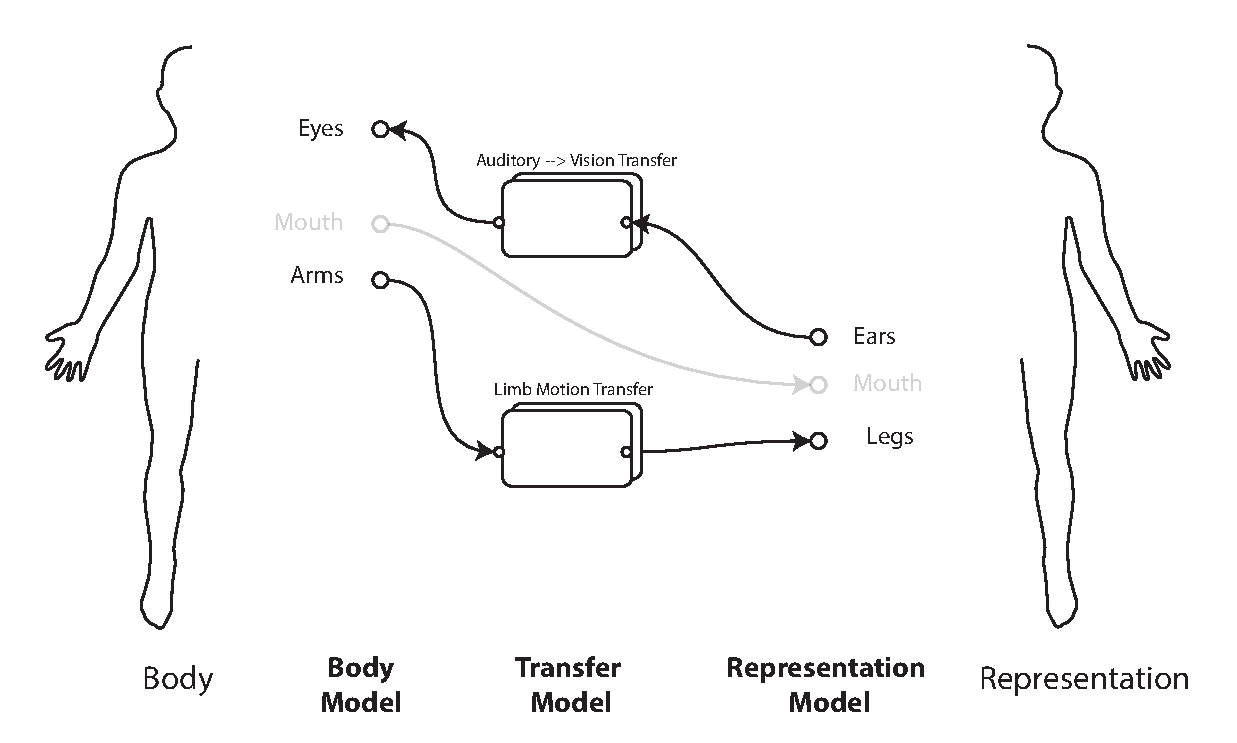
\includegraphics[width=1\textwidth]{figures/concept/EDD-Top.pdf}
\caption{Topology reconfiguration meta-modeling.}
  \label{fig:concept-EDD-TopRec}
\end{figure}

When physical limitation prevents certain modalities to be used, or when a new bodily function that is not driven from the human body in the representation requires matching with operator body, then the design process is focused on the body topology side. Topology Reconfiguration design category focuses on altering the postural modality data flow from the user side and mapping it into the intended representation. This design category can be used to enable physically impaired users or people with lost limbs to alter their body schema and use different functional limb as a substitution for a modality. For example, a mobility impaired person (cannot walk), can use his head motion as an alternative method in order to navigate using the remote representation. This would provide direct and embodied operation, and would require a minimum amount of training to use.

To illustrate this meta-model design pattern, \Figure{fig:concept-EDD-TopRec} shows an example of reconfiguring body topology (postural and sensory topologies) by redirecting the mapping of the body's modalities into different modalities in the representation. To achieve such mapping, transfer blocks are required to translate the information flow between such modalities. For example, sensory substitution can be considered as topology reconfiguration, in which one sensory organ is mapped into another by converting the source information into the target modality. 

There are considerations when topology reconfiguration is intended to be used. Certain modalities should not be arbitrarily mapped to a different one. For example, mapping wrist tilts rotational axis into panning axis of the head motion. This type of modulation would cause disembodiment although the motion is driven by the wrist. To avoid such disembodiment cases, its possible to define set of constraints on the joints channel mapping:
\begin{itemize}
\item \textbf{Rotational mapping}: Joint axes should be mapped as:
\begin{equation}
\begin{split}
DestJ_{tilt} &=F_{A}(SrcJ_{tilt}) \\
DestJ_{pan} &=F_{B}(SrcJ_{pan}) \\
DestJ_{roll} &=F_{C}(SrcJ_{roll})
\end{split}
\end{equation}
$SrcJ $: Source joint (driving joint from the user side).\\
$DestJ$: Destination joint (target joint at the representation side).\\
$F_{A},F_{B},F_{C}$: are functions that can be applied on each individual axis to alter the motion (e.g. linear mapping $F(X)=X$)

\item \textbf{Spatial mapping}: Similarly to rotational mapping constraint, the spatial mapping constraint the mapping between axes (X,Y,Z) to the corresponding ones in the destination.

\item \textbf{Directional mapping}: The spatial and rotational mapping should follow the sign of the source motion (not to use inverse function on the joint motion).

%Side mapping (left--> right) [Need references]
\end{itemize}

In summary, this design pattern is intended to remap body modalities into different ones in order to overcome a physical disability imposed by a certain modality. This design pattern can be combined with other meta-modeling design patterns when designing a system.

%To highlight the meta-model process for topology reconfiguration, a scenario is described here. The representation system used is an ordinary telexistence system as shown in \Figure{fig:concept-EDD-Redirected}. The user side, however, can not use head rotation due to physical limitations, and thus a different postural modality to be used. In this example, the user wants to operate the head motion using his eye gaze motion, so when the user looks left, the robot head starts to pan to the left side, and vise-versa for the right side. Similarly, looking up would tilt the head to up, and vise-versa for the bottom. The motion mapping follows the constraints described previously. For this meta-model, an [Eye Gaze] perceptual block is used to measure the pupil position of the user, and it outputs a 2D vector (X,Y) describing the pupil looking location along the horizontal and vertical axes as value range of [-1,1] for each axis. To translate this vector into a rotational joint output, a [Motion Transfer] block can be used. It converts an input vector into tilt and pan rotation, which then can be linked into a destination joint. The output of [Motion Transfer] block is linked into [Head Rotation] at the representation model.




\subsection{Modality Expansion}
\label{sec:concept-ModAlt}
%\protect\footnote{For further details regarding Layered Presence, please refer to author's papers \cite{saraiji2016layered,saraiji2016study}}}


\begin{figure}[htpb]
  \centering
  \captionsetup{justification=centering}
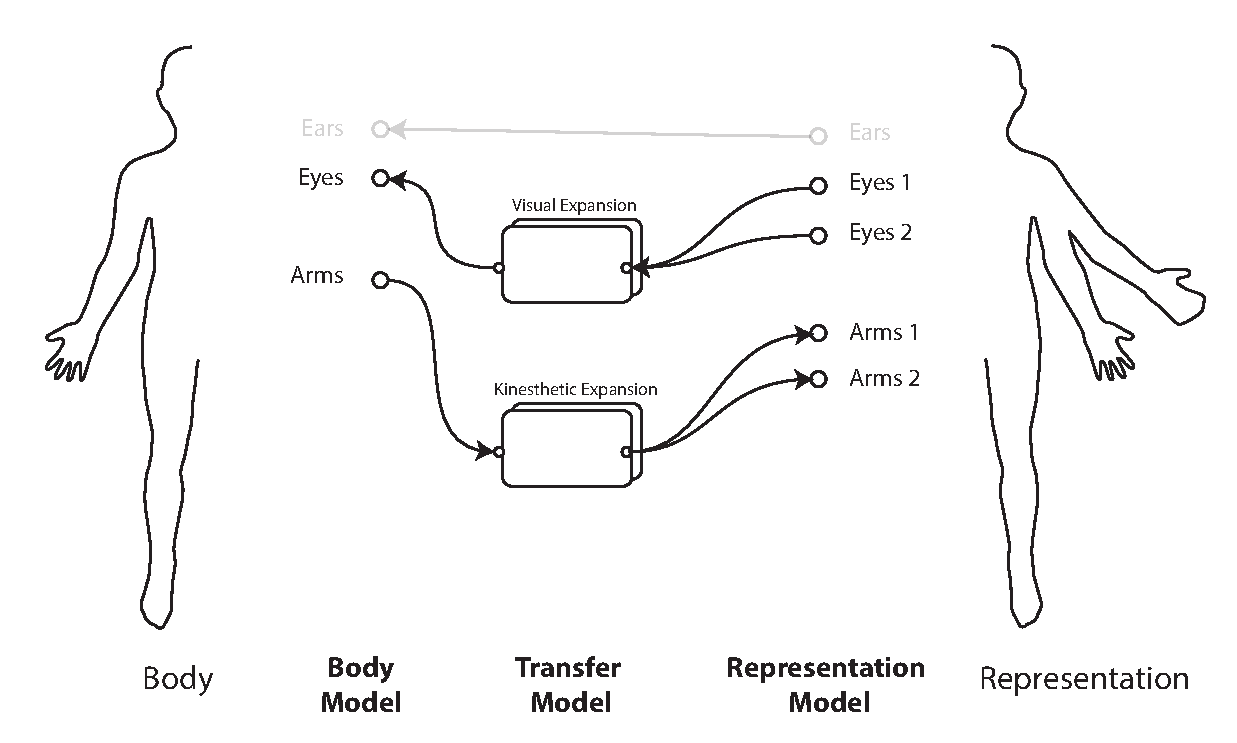
\includegraphics[width=1\textwidth]{figures/concept/EDD-Expansion.pdf}
\caption{Modality expansion meta-modeling.}
  \label{fig:concept-EDD-ModExp}
\end{figure}

The previously proposed design patterns have mainly addressed direct one-to-one body schema mapping in which each body modality communicates with a single modality at a time. In that type of systems, the sensory and postural topologies are constrained to a single representation. \textit{Modality Expansion} design pattern addresses systems with non-linear mapping, that is the operator can access multiple modalities and receives feedback from them, or controls them simultaneously. This control and feedback mechanisms in this meta-model should address the following considerations:
\begin{itemize}
  	\setlength\itemsep{0em}
    \item Real-time simultaneous representation of body, visuals, and auditory feedback in multiple locations.
    \item Natural mechanism of presenting the visuals from the multiple sources to human user.
    \item Intuitive mechanism for switching the visual perception between the locations, while maintaining the awareness of the other locations.  
\end{itemize}

To illustrate this design pattern, \Figure{fig:concept-EDD-ModExp} shows mapping body modalities into multiple modalities in the representation. The representation can be single with multiple modalities, or several representations that the user connects to and controls simultaneously. 

To design a meta-model that can provide such non-linear mapping of body topology and representation topology, the concept of ``Modality Layer'' is used. The layer contains both the postural and perceptual modalities of the representation used, and thus when $N$ modalities are required to interact with, we would have $N$ layers [$L_{1}...L_{N}$] that are derived from these modalities. These layers are aggregated together to produce the input to the perceptual or postural modalities of the user. These layers can be mixed (or blended) and delivered to the user and representation using corresponding transfer blocks.

This design pattern helps to expand body's limitations to perceive and control multiple representations that can be located locally, or connected remotely (ubiquitous).

%This method can be expanded to more than just Telexistence related applications. By using the concept of layering, its possible to generalize the layers to be media or even interactive applications, and apply the same procedure in combining them into a single space. 



\pagebreak

\section{Physical Embodiment Toolkit}
\label{concept:toolkit}
%describe the goal of the embodiment toolkit

In order to facilitate the process of prototyping meta-models and experiment the effect of altering the mapping of various modalities, an embodiment toolkit is proposed. The toolkit is a general purpose physical representation designed in a robotic form, which provides essential modalities to access through EDD framework. This toolkit can be looked as being a tool to reprogram our bodies and our presence. The design considerations for this proposed toolkit are described in this section. 

For this thesis, this toolkit was used completely or partially in several projects (discussed in \Chapter{ch:eval}) and provided an agile design and testing process for these projects.

\subsection{Human Driven Design}

Human bodies provide high degree of complexity and constraints. The toolkit should provide a balance between the complexity of replicating the human body structure and the affordability to create a general purpose system. The following modalities are mainly considered to be available in the design of the hardware:

\begin{itemize}
\item \textbf{Vision feedback}: as in teleoperation and presence applications, the main sensory feedback we would rely on to gather information about the surrounding environment is the vision, or the eyes. The representation should provide means of capturing real-time visuals and provide them in bodily acceptable format, that is a stereo vision. As in Telexistence systems, stereo vision is an important design consideration that is required by the slave system to provide. For general use case purpose, the interpupillary distance (IPD) for the vision system is to be fixed on an average of 64mm \cite{dodgson2004variation}. Field of vision should be wide enough to cover at least $60\deg$ of user's field of view, so the user can obtain feedback from the peripheral vision. The visual feedback should provide real-time feedback with corrected distortion in order to avoid ``Motion Sickness'' cases, that is, the disagreement between visually perceived optical flow and motion, and the vestibular system's sense of movement which caused the motion. In this thesis, the latency considerations should be less than 100ms for the visual system. The responsiveness (or framerate) of the vision system should be high enough to minimize the motion sickness as well as balanced to maintain low latency feedback (the higher the framerate, the more performance demand from the system is required, and thus higher latency will occur). Within these constraints, the spatial resolution of the images can be considered depending on the target application (for teleoperation and inspection purpose, low resolution can be sufficient to be used).

To use in EDD, the toolkit should expose a block that provides access to the eyes modality of the representation. In the representation model category, [Eyes] block is used to output stereo visual data channel from the toolkit into the meta-model.

\item \textbf{Auditory feedback}: The auditory system of human body is an important cue to have spatial awareness of the events occurring around. The binaural feedback provides an understanding of the sound sources locations. For this modality, the system should provide a similar experience of human ears. To maintain high auditory spectrum feedback, the audio system should provide high-frequency sampling of the audio. Human ears can perceive a range of 20Hz to 20,000Hz of auditory spectrum. Thus the sampling rate should be at least twice the frequency (based on Nyquist–Shannon sampling theorem), so 40,000Hz audio sampling is the minimum requirement for the audio system. The closest supported standard audio frequency by the hardware is 44,100Hz. The audio transmission should be synchronized with the visual feedback in order to avoid any disengagement of visual-auditory cross-modality during operation. 

The auditory feedback is integrated into EDD framework by providing [Ears] block under representation model category to output binaural audio data channel from the toolkit into the meta-model. 

\item \textbf{Verbal communication}: Since the representation is generally used as a replication of human body, auditory communication system would be required to provide bi-directional audio from/to the toolkit along with the auditory feedback system. The design verbal communication system has fewer constraints than the previous modalities. Single audio channel output is sufficient to be included in the toolkit design. For frequency considerations, this channel mainly transmits the verbal audio from the human operator, thus the frequency sampling can be less than the auditory feedback channels. Old telecommunication systems (such as the telephone) used 8,000Hz sampling rate, although it was sufficient for human speech however it cannot support sibilance (ess/s/ and eff/f/ sounds ). To overcome this, Wideband frequency 16,000Hz sampling rate is considered for the transmission and playback.

In EDD framework, under representation model category, a [Mouth] block is provided by the toolkit to communicate the auditory data channel from the meta-model to the representation hardware. 

\item \textbf{Postural design}: the mechanical structure of the toolkit reflects the degrees of freedom (DOF) and limits of the operation and mapping with the user. The postural schema of the toolkit should provide visual-kinesthetic cross-modality, thus a structure that mimics the head motion is needed. A three DOF head structure would provide rotational motion along the tilt, pan, and roll axes are sufficient to produce the motion for the eyes. Speed and joints acceleration of the head design is required to match the speed and acceleration of human neck. If an inadequate speed and resolution were used, the system would result in mechanical latency and thus motion sickness would occur. To address these speed limitations, a user-study is required to calculate the maximum rotational speed of human neck. 

For the parallax motion of the upper body, the addition of three extra DOF would provide the lower motion of the human torso \cite{watanabe2008torso}. However, the usage of these extra joints would increase the size and affordability of the toolkit. The addition of these DOFs is optional, and is application specific. Two versions of the toolkit can be designed: Head only (3DOF) and Head+Parallax (6DOF).

The postural modalities are exposed into EDD under representation model category as a set of blocks representing the body. For the neck modality, the [Neck Joint] block is used to communicate the target head orientation and position (if parallax motion was required).

\end{itemize}

\subsection{Extensibility and Modularity}
Although the toolkit provides a minimal amount of modalities as described in the previous point, however, it should also support the ability to modify and extend its functions by integrating new types of modalities into it. A modular design is considered for both the software and the hardware. The design of the software architecture on the toolkit should be capable to handle the addition of new types of functions, while maintaining the existing ones,e.g. adding an extra set of vision module into the toolkit. A common use case for such modularity is the haptic sensors. The number of haptic sensors can vary depending on the application, for example, its possible to integrate a tactile sensor on the bottom of the toolkit to capture the ambient vibrations of the location the toolkit is placed at (table top for example). 

For each of the newly added modules, a separate information channel is generated to communicate with the EDD model. Also, a dedicated block is to be designed and integrated into the representation model (defined by \textit{Representation engineer}).

\subsection{Accessibility}

In order to design remote presence alteration experiences using EDD meta-modeling, the toolkit should provide network accessibility. Thus, all the communications between the toolkit and the user side should be carried over dedicated network channels and in a digitized format. The network medium can be done through wired local area networks (Ethernet), or a wireless medium (e.g. Wi-Fi IEEE 802.11 standard) in cases such as mobility is required. This design consideration helps to allow flexibility in connecting to the toolkit, either as a single toolkit at a time, or multiple toolkits simultaneously. 

\section{Design Summary}

This chapter has introduced the overall concept of Embodied-Driven Design (EDD) and meta-modeling design process. EDD derives the various modalities of the human body in a loosely, hierarchical structure in order to engineer a mapping between a human body and an alternative representation, such as telexistence system. This loosely representation helps to alter the input and output of the modalities, or remap them with non-corresponding modalities at the representation side. Meta-modeling is the process of defining body schema mapping by using various types of perceptual, transfer, and representation blocks. Four meta-modeling design categories were described: Direct body transfer, Representation alteration, Topology reconfiguration, and Modality expansion. These categories provide the design process for the systems that will be discussed in \Chapter{ch:eval}. However, EDD is not limited to these meta-models design categories. To expand the usability and utility of EDD, a physical embodiment toolkit is proposed that it can be used along with modeling framework to achieve customizable body mapping and interaction alterations. This toolkit is also used in the projects discussed within this thesis.




